\section{Introduction}\label{sec:introduction-results}
This section is describing experiments results with different conditions
for Kafka Streams and Apache Flink.
For each experiment, the following parameters are used:

\begin{description}
    \item[Experiment execution time] 18 minutes
    \item[Messages per second] 200000
    \item[Message size] 1KB
    \item[Number of Kafka topic partitions] 50
    \item[Worker killing period] 3 minutes
    \item[Number of states] 20000
    \item[Selectivity] 50\%
\end{description}


These experiments that were running for this case study:

\begin{itemize}
    \item Kafka Streams with having 8 worker replicas killed every 3 minutes
    \item Kafka Streams with having 2 worker replicas killed every 3 minutes
    \item Apache Flink with having 2 worker replicas killed every 3 minutes
    \item Apache Flink with having 8 worker replicas killed every 3 minutes
\end{itemize}


\newpage
\section{Benchmarking Kafka Streams Fault Tolerance}\label{sec:benchmarking-kafka-streams-fault-tolerance}

\subsection{Analyzing 2-Pod Failures in an 8-Pod Cluster}\label{subsec:analyzing-2-pod-failures-in-an-8-pod-cluster}


\begin{figure}[ht]
    \centering
    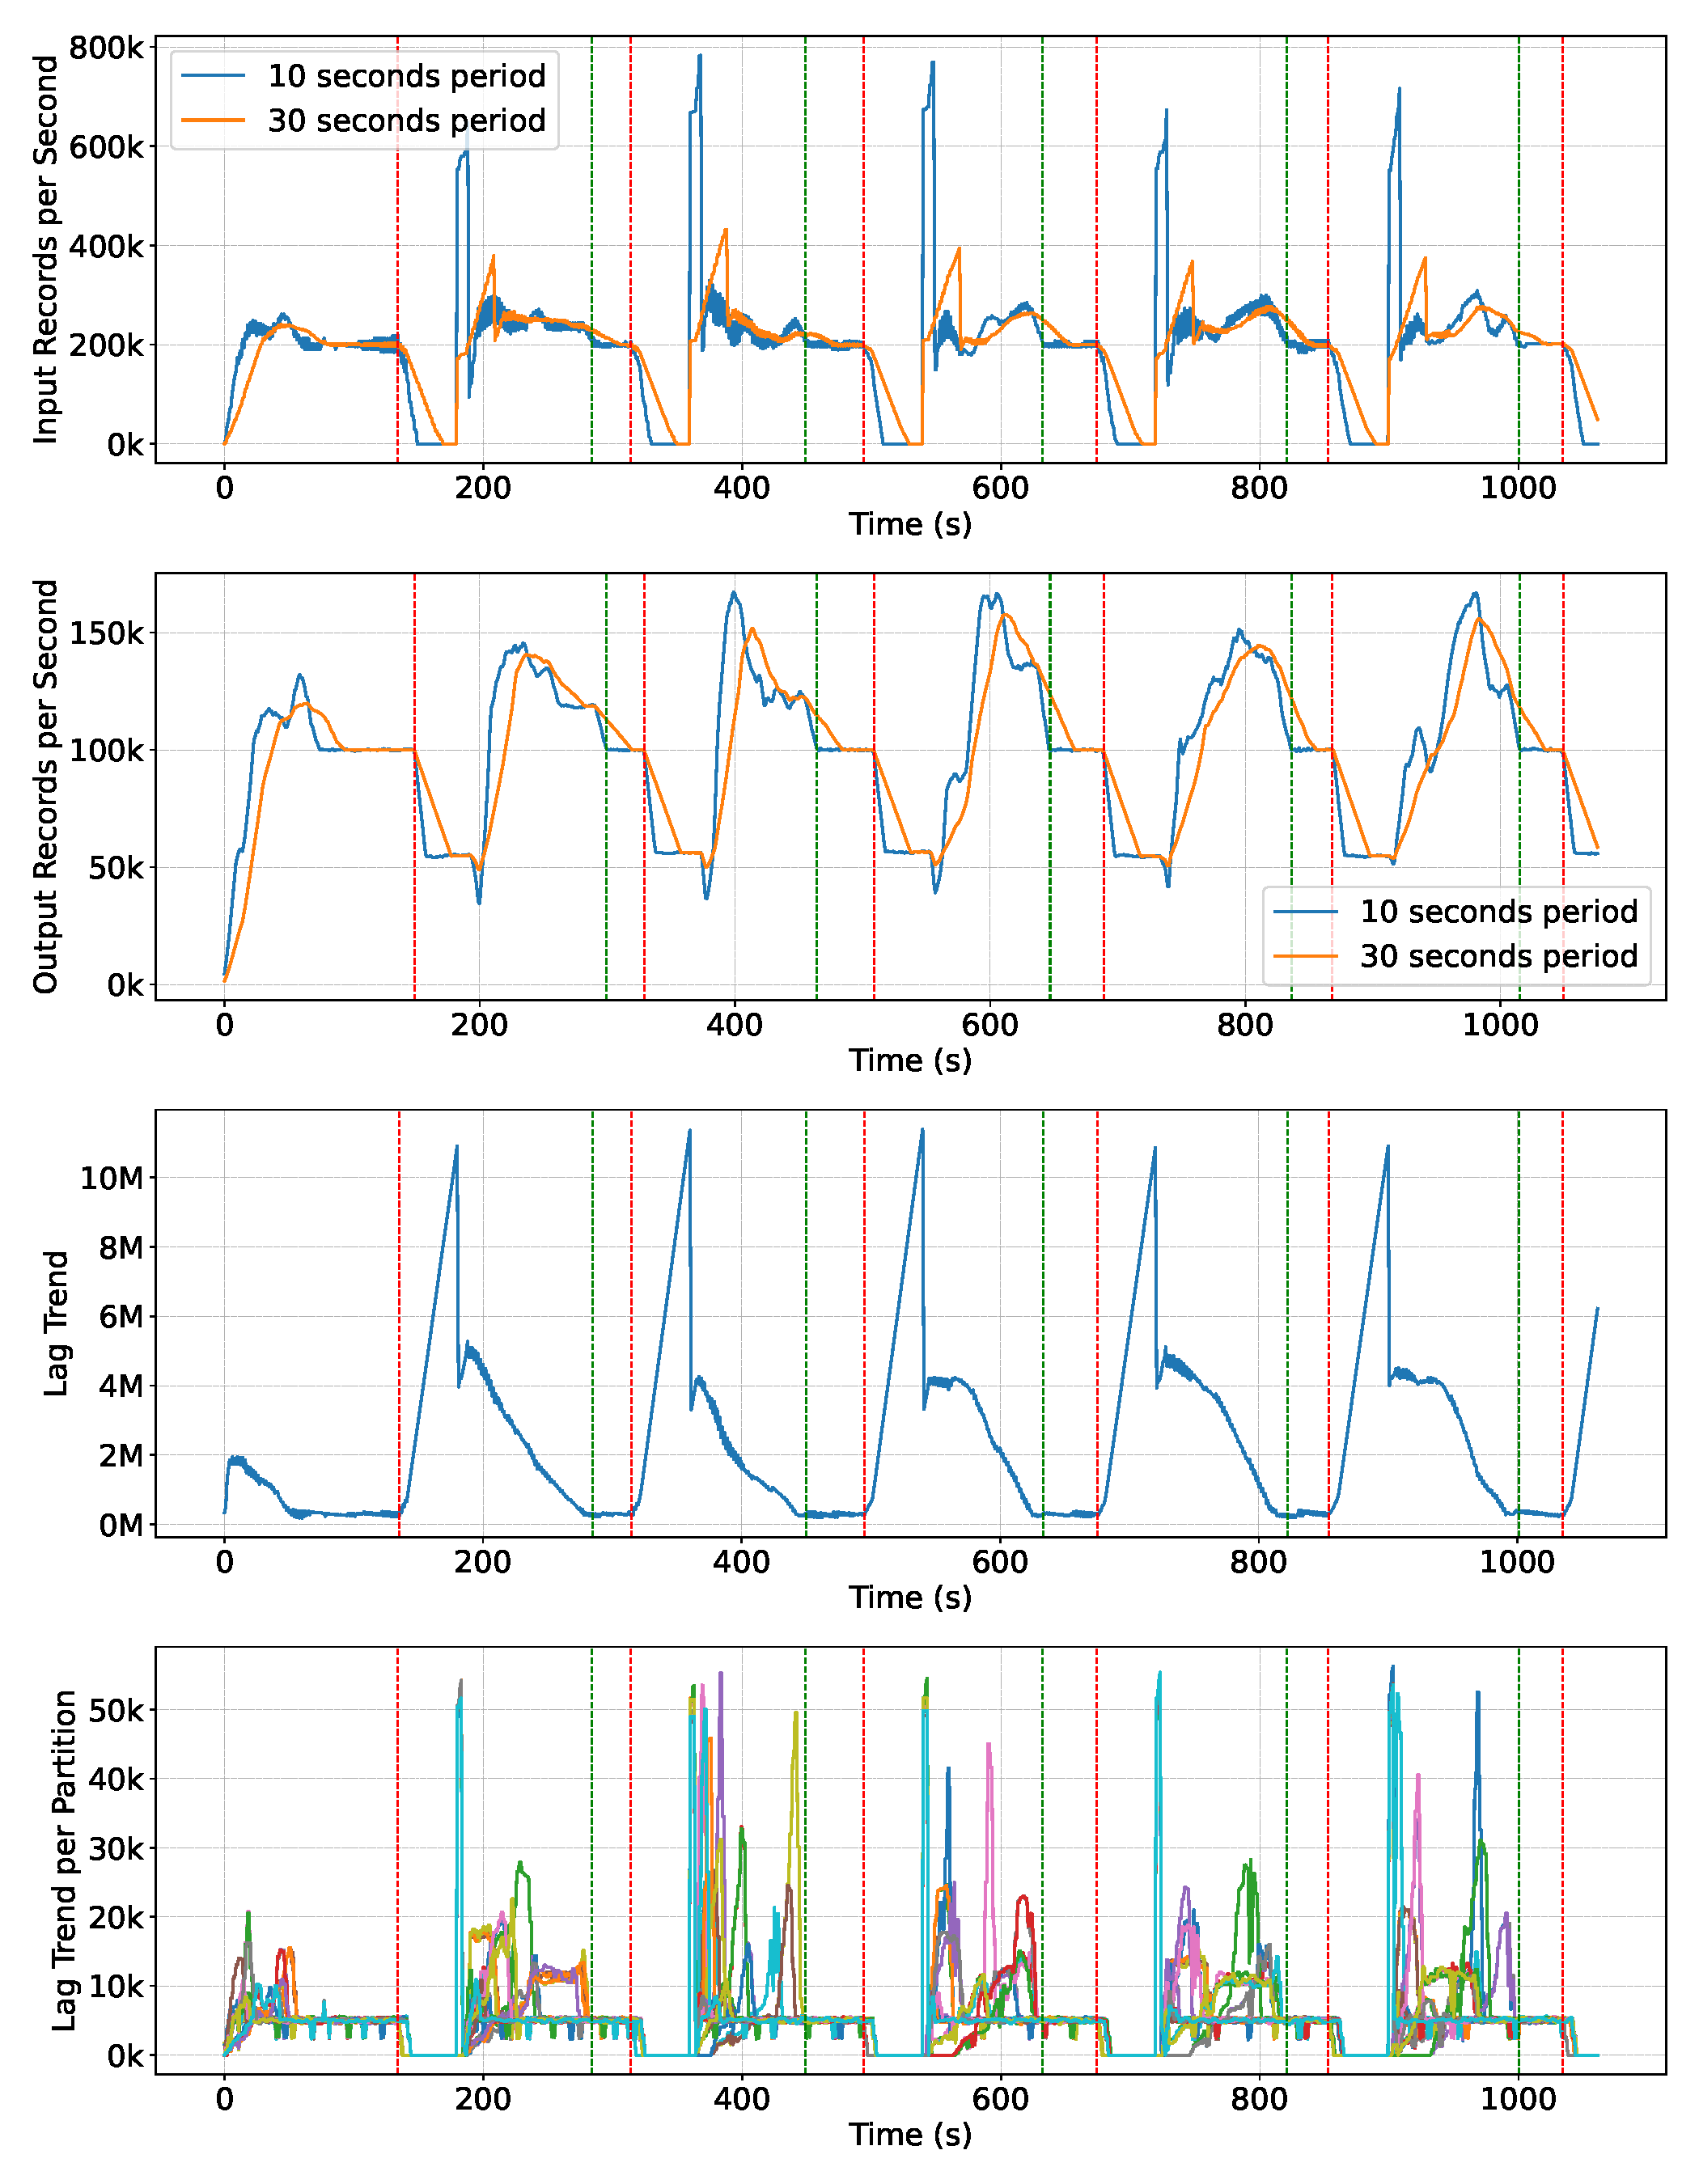
\includegraphics[width=1\textwidth]{figures/kstreams-2pods/kafka_2_pods_plot_impact}
    \caption{\textit{Text.}}
    \label{fig:kafka-2pods-impact}
\end{figure}


\begin{figure}[ht]
    \centering
    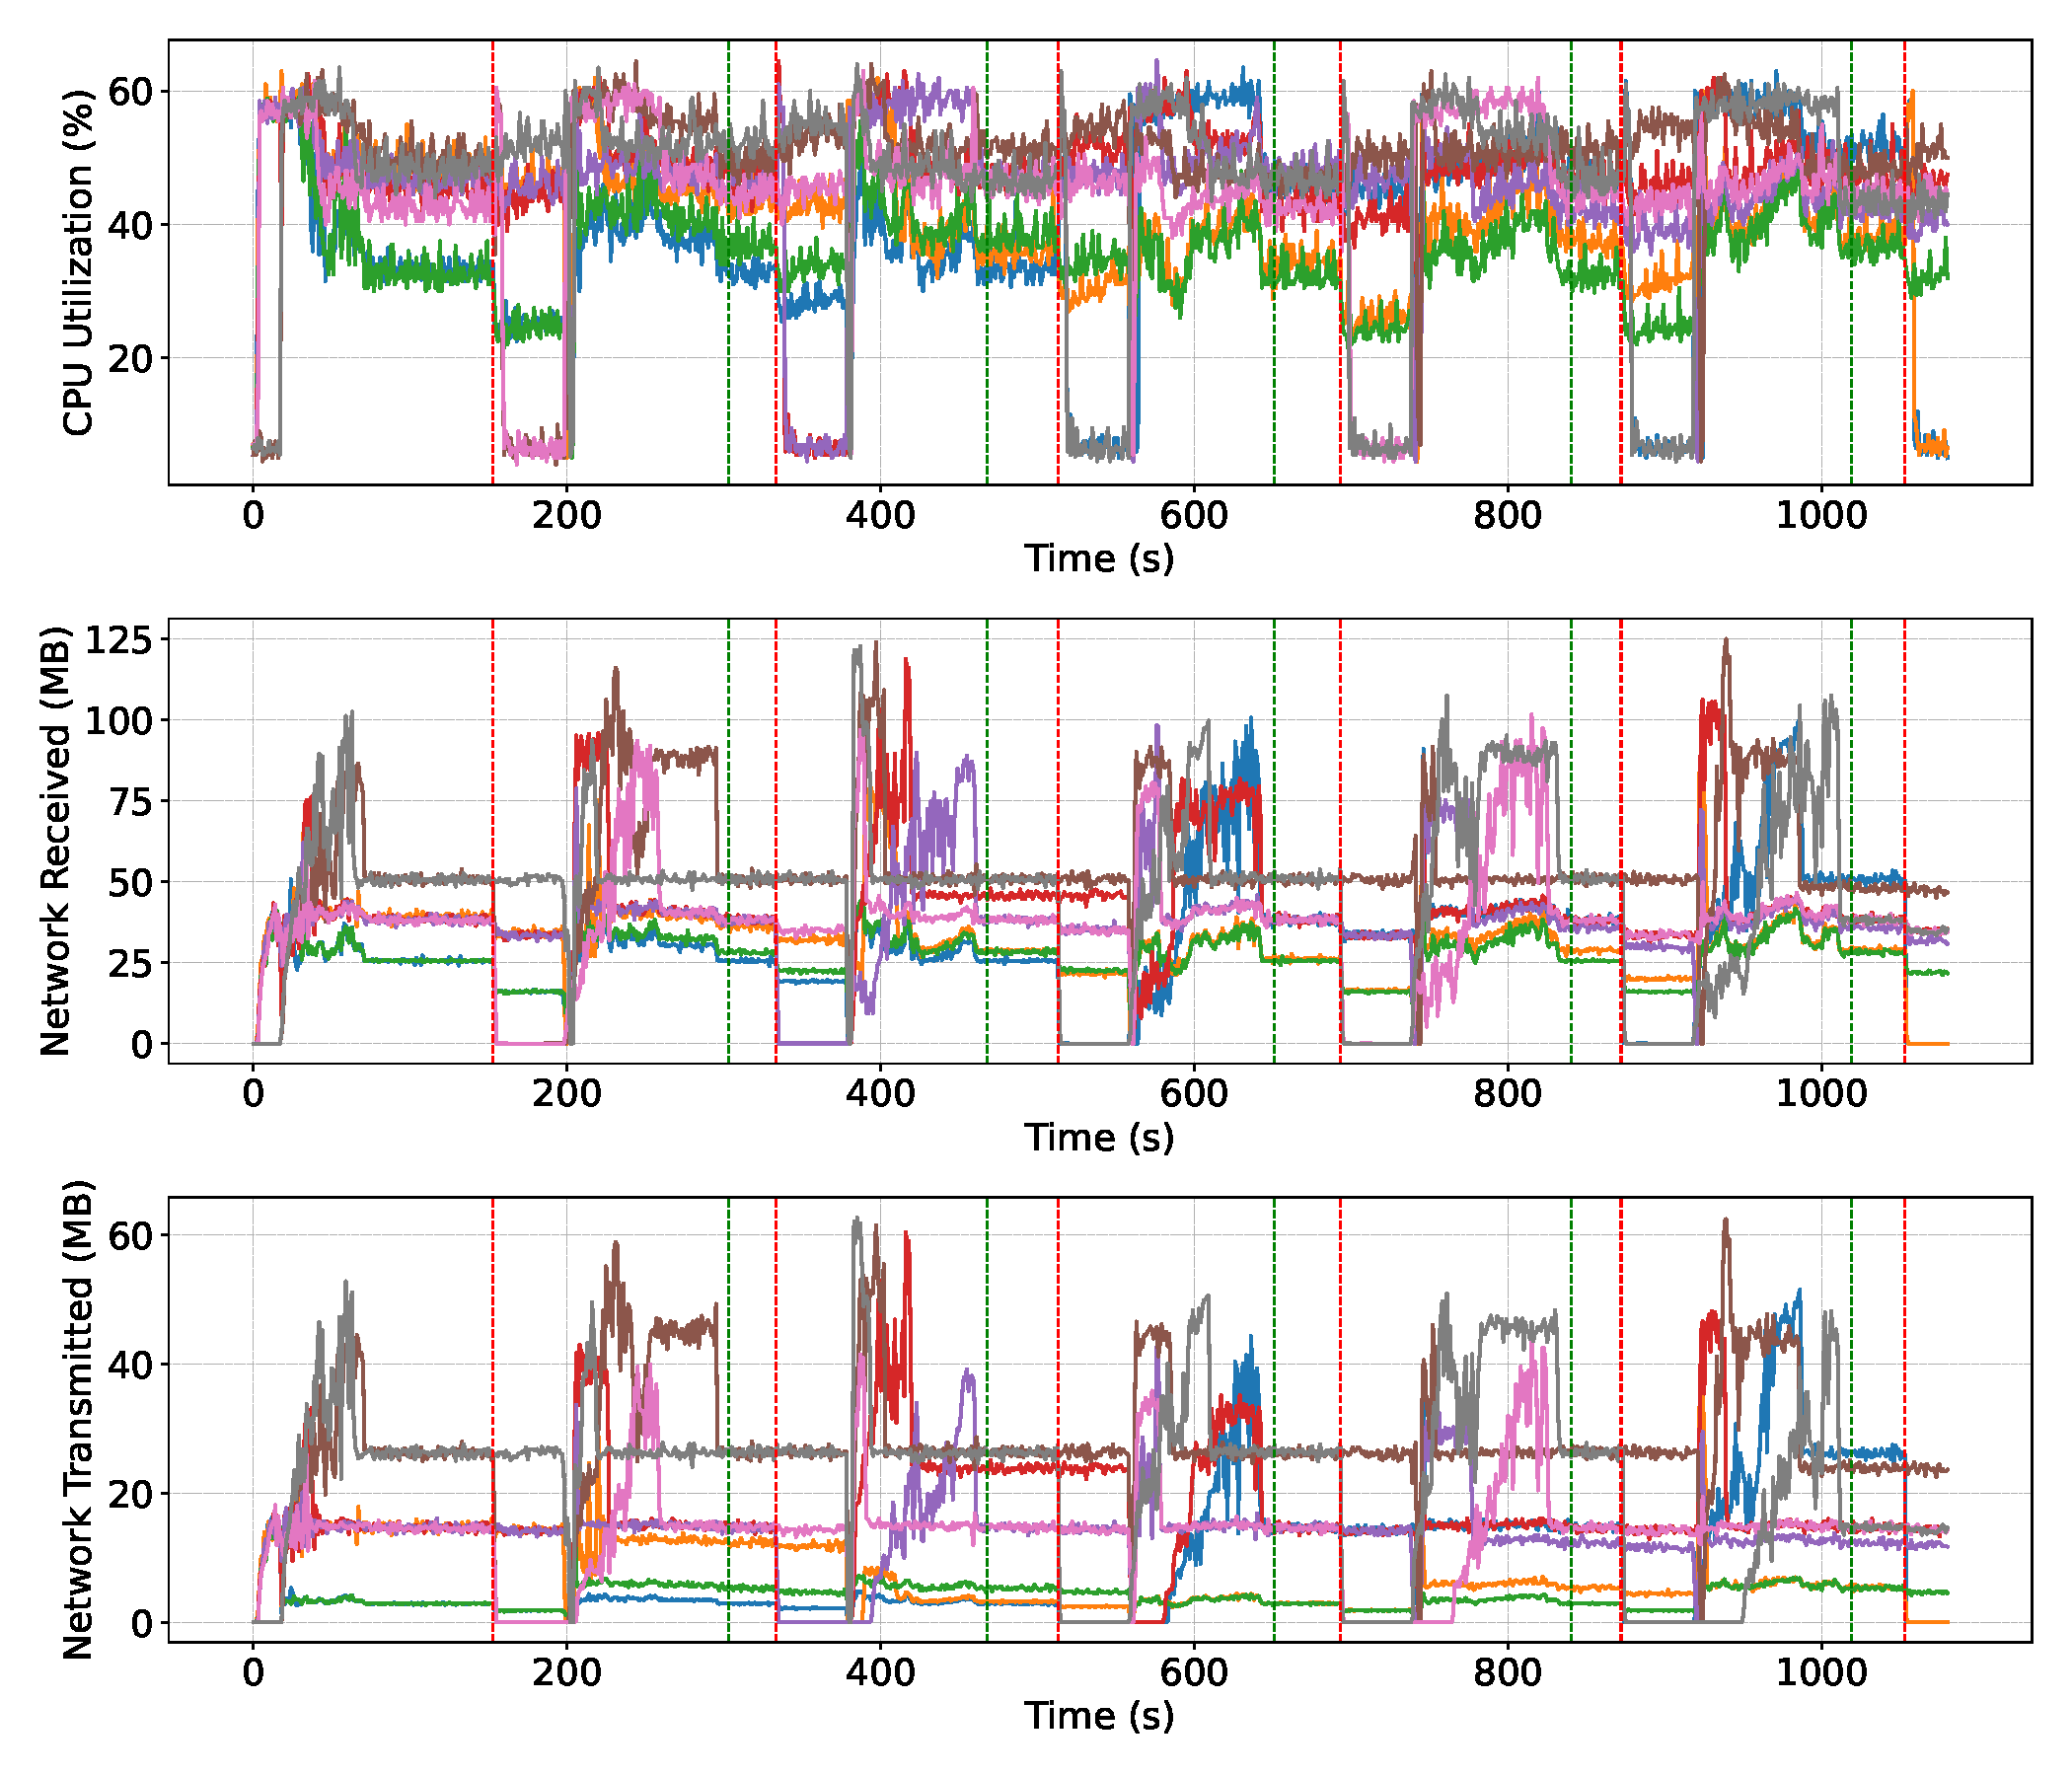
\includegraphics[width=1\textwidth]{figures/kstreams-2pods/kafka_2_pods_resources}
    \caption{\textit{Text.}}
    \label{fig:kafka-2pods-resource}
\end{figure}


\subsection{Analyzing 8-Pod Failures in an 8-Pod Cluster}\label{subsec:analyzing-8-pod-failures-in-an-8-pod-cluster}

\begin{figure}[ht]
    \centering
    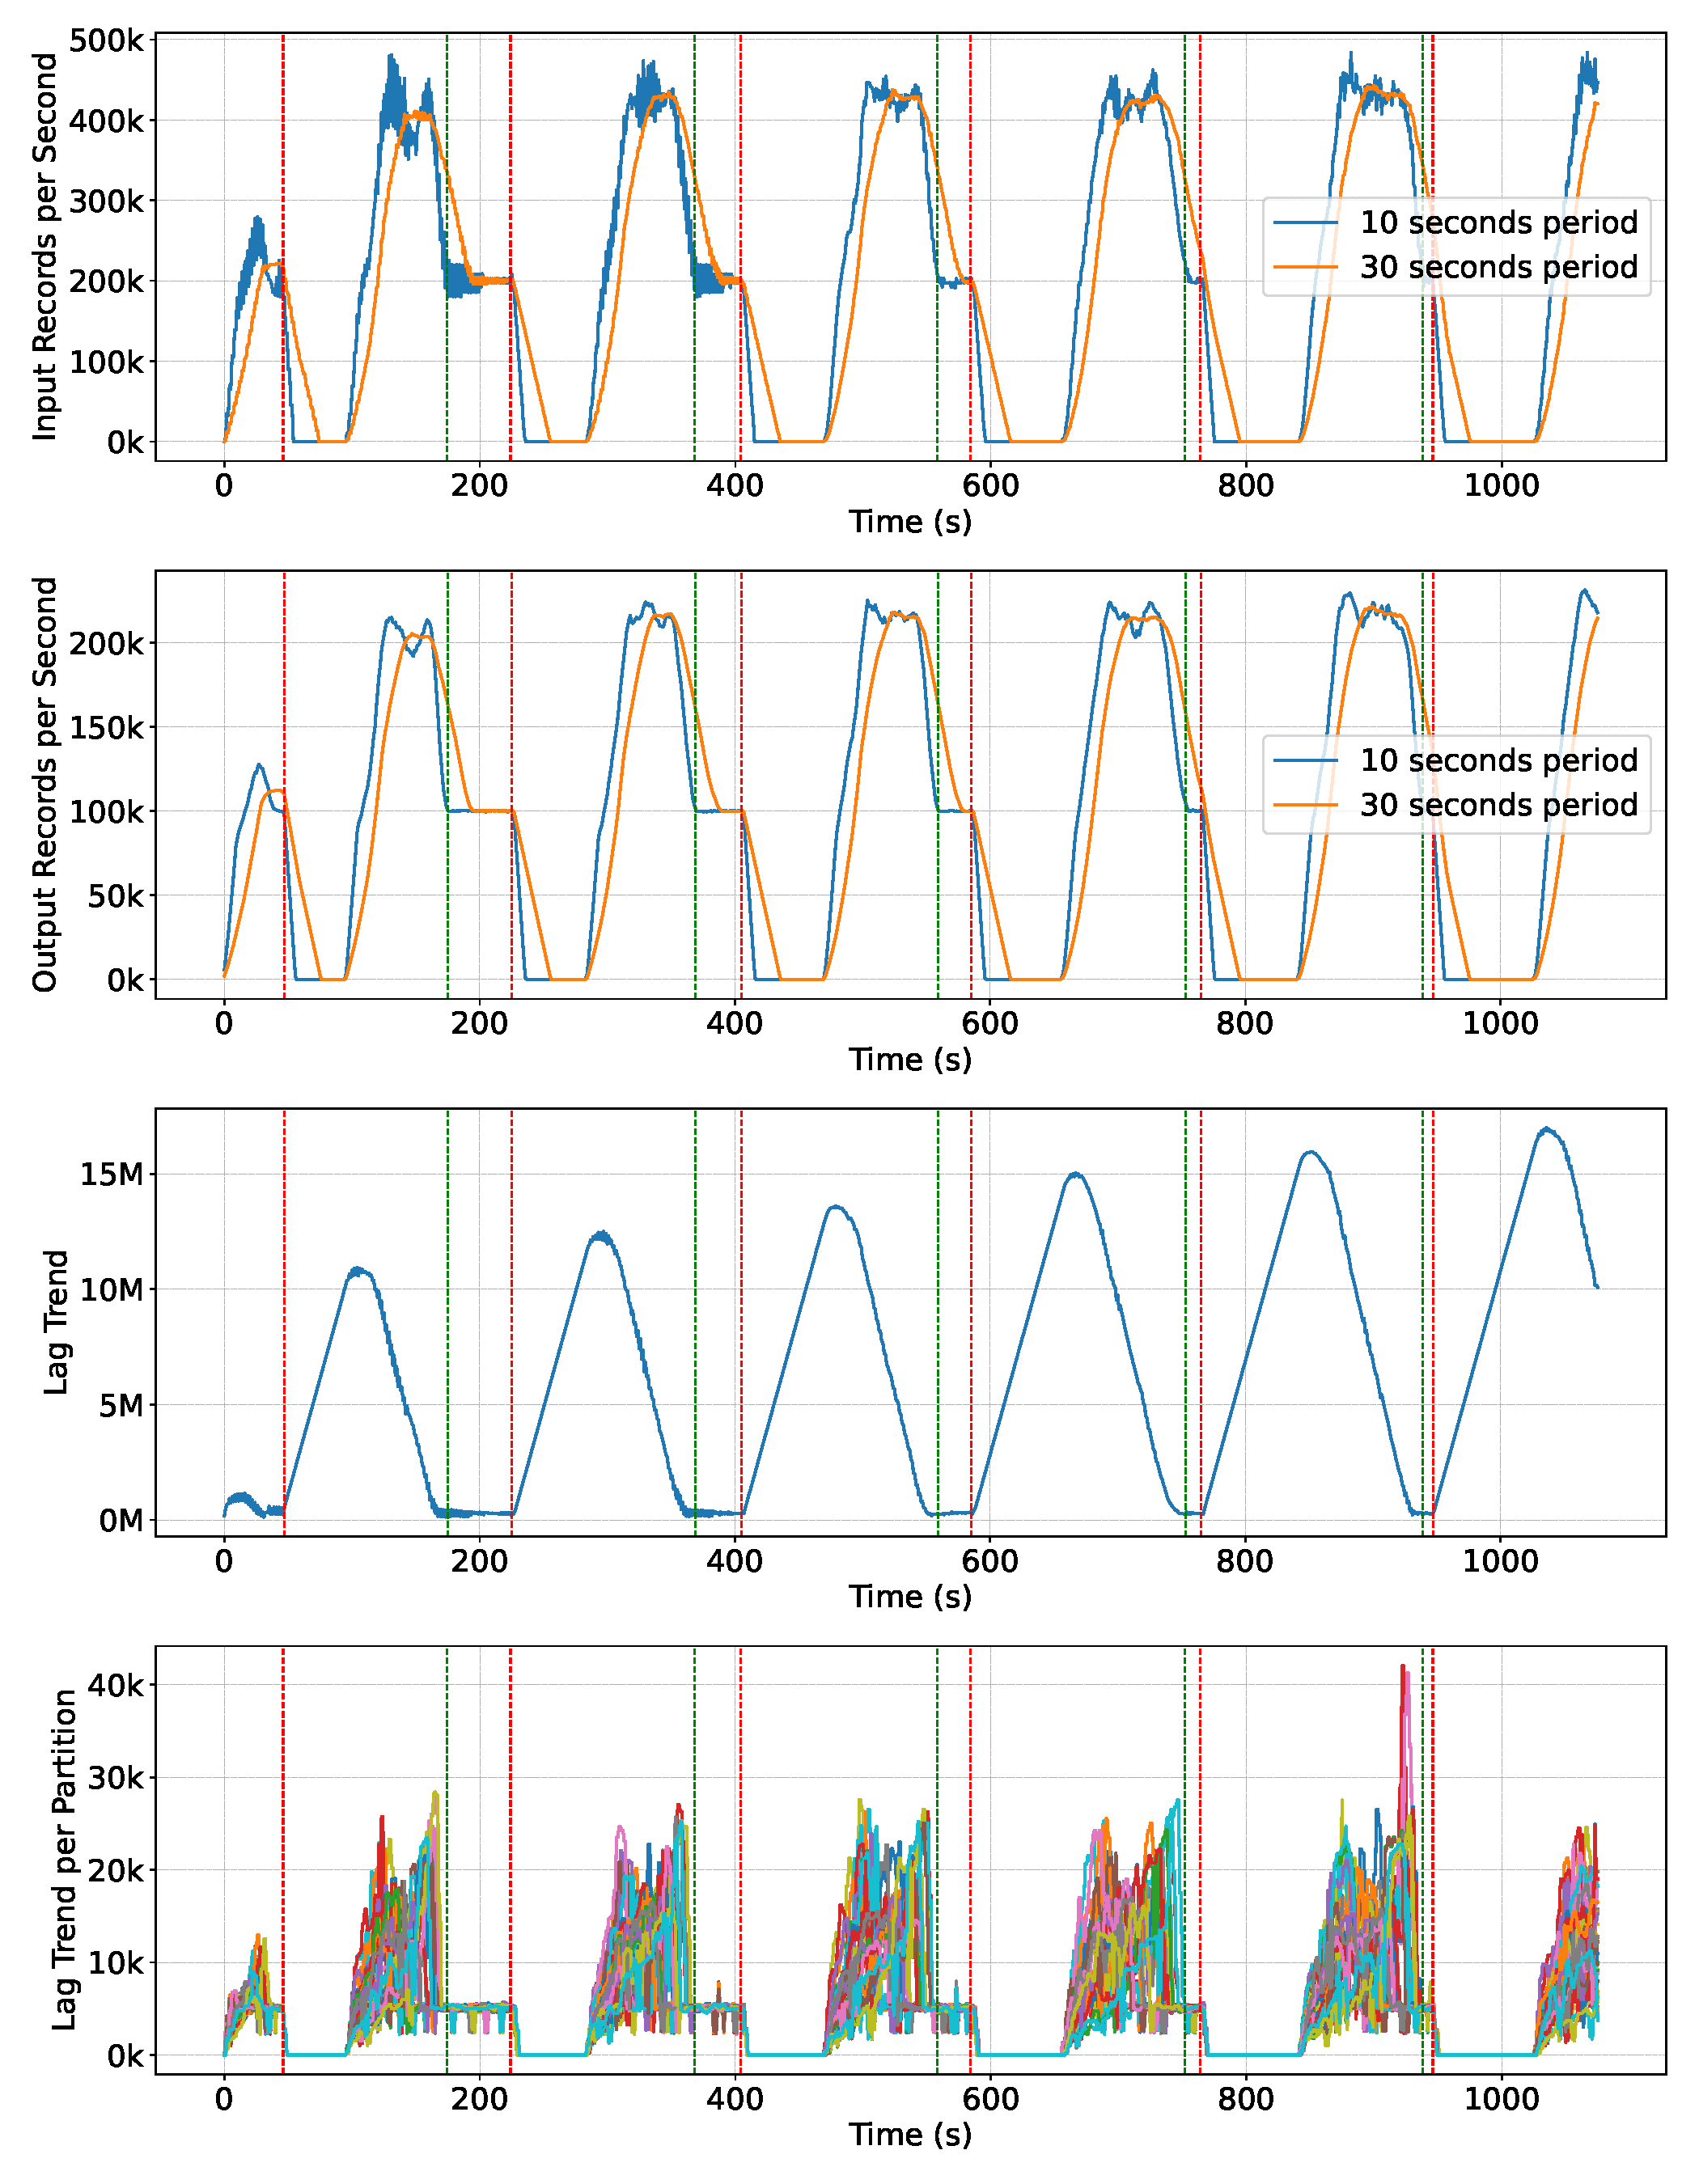
\includegraphics[width=1\textwidth]{figures/kstreams-8pods/kafka_8_pods_plot_impact}
    \caption{\textit{Text.}}
    \label{fig:kafka-8pods-impact}
\end{figure}


\begin{figure}[ht]
    \centering
    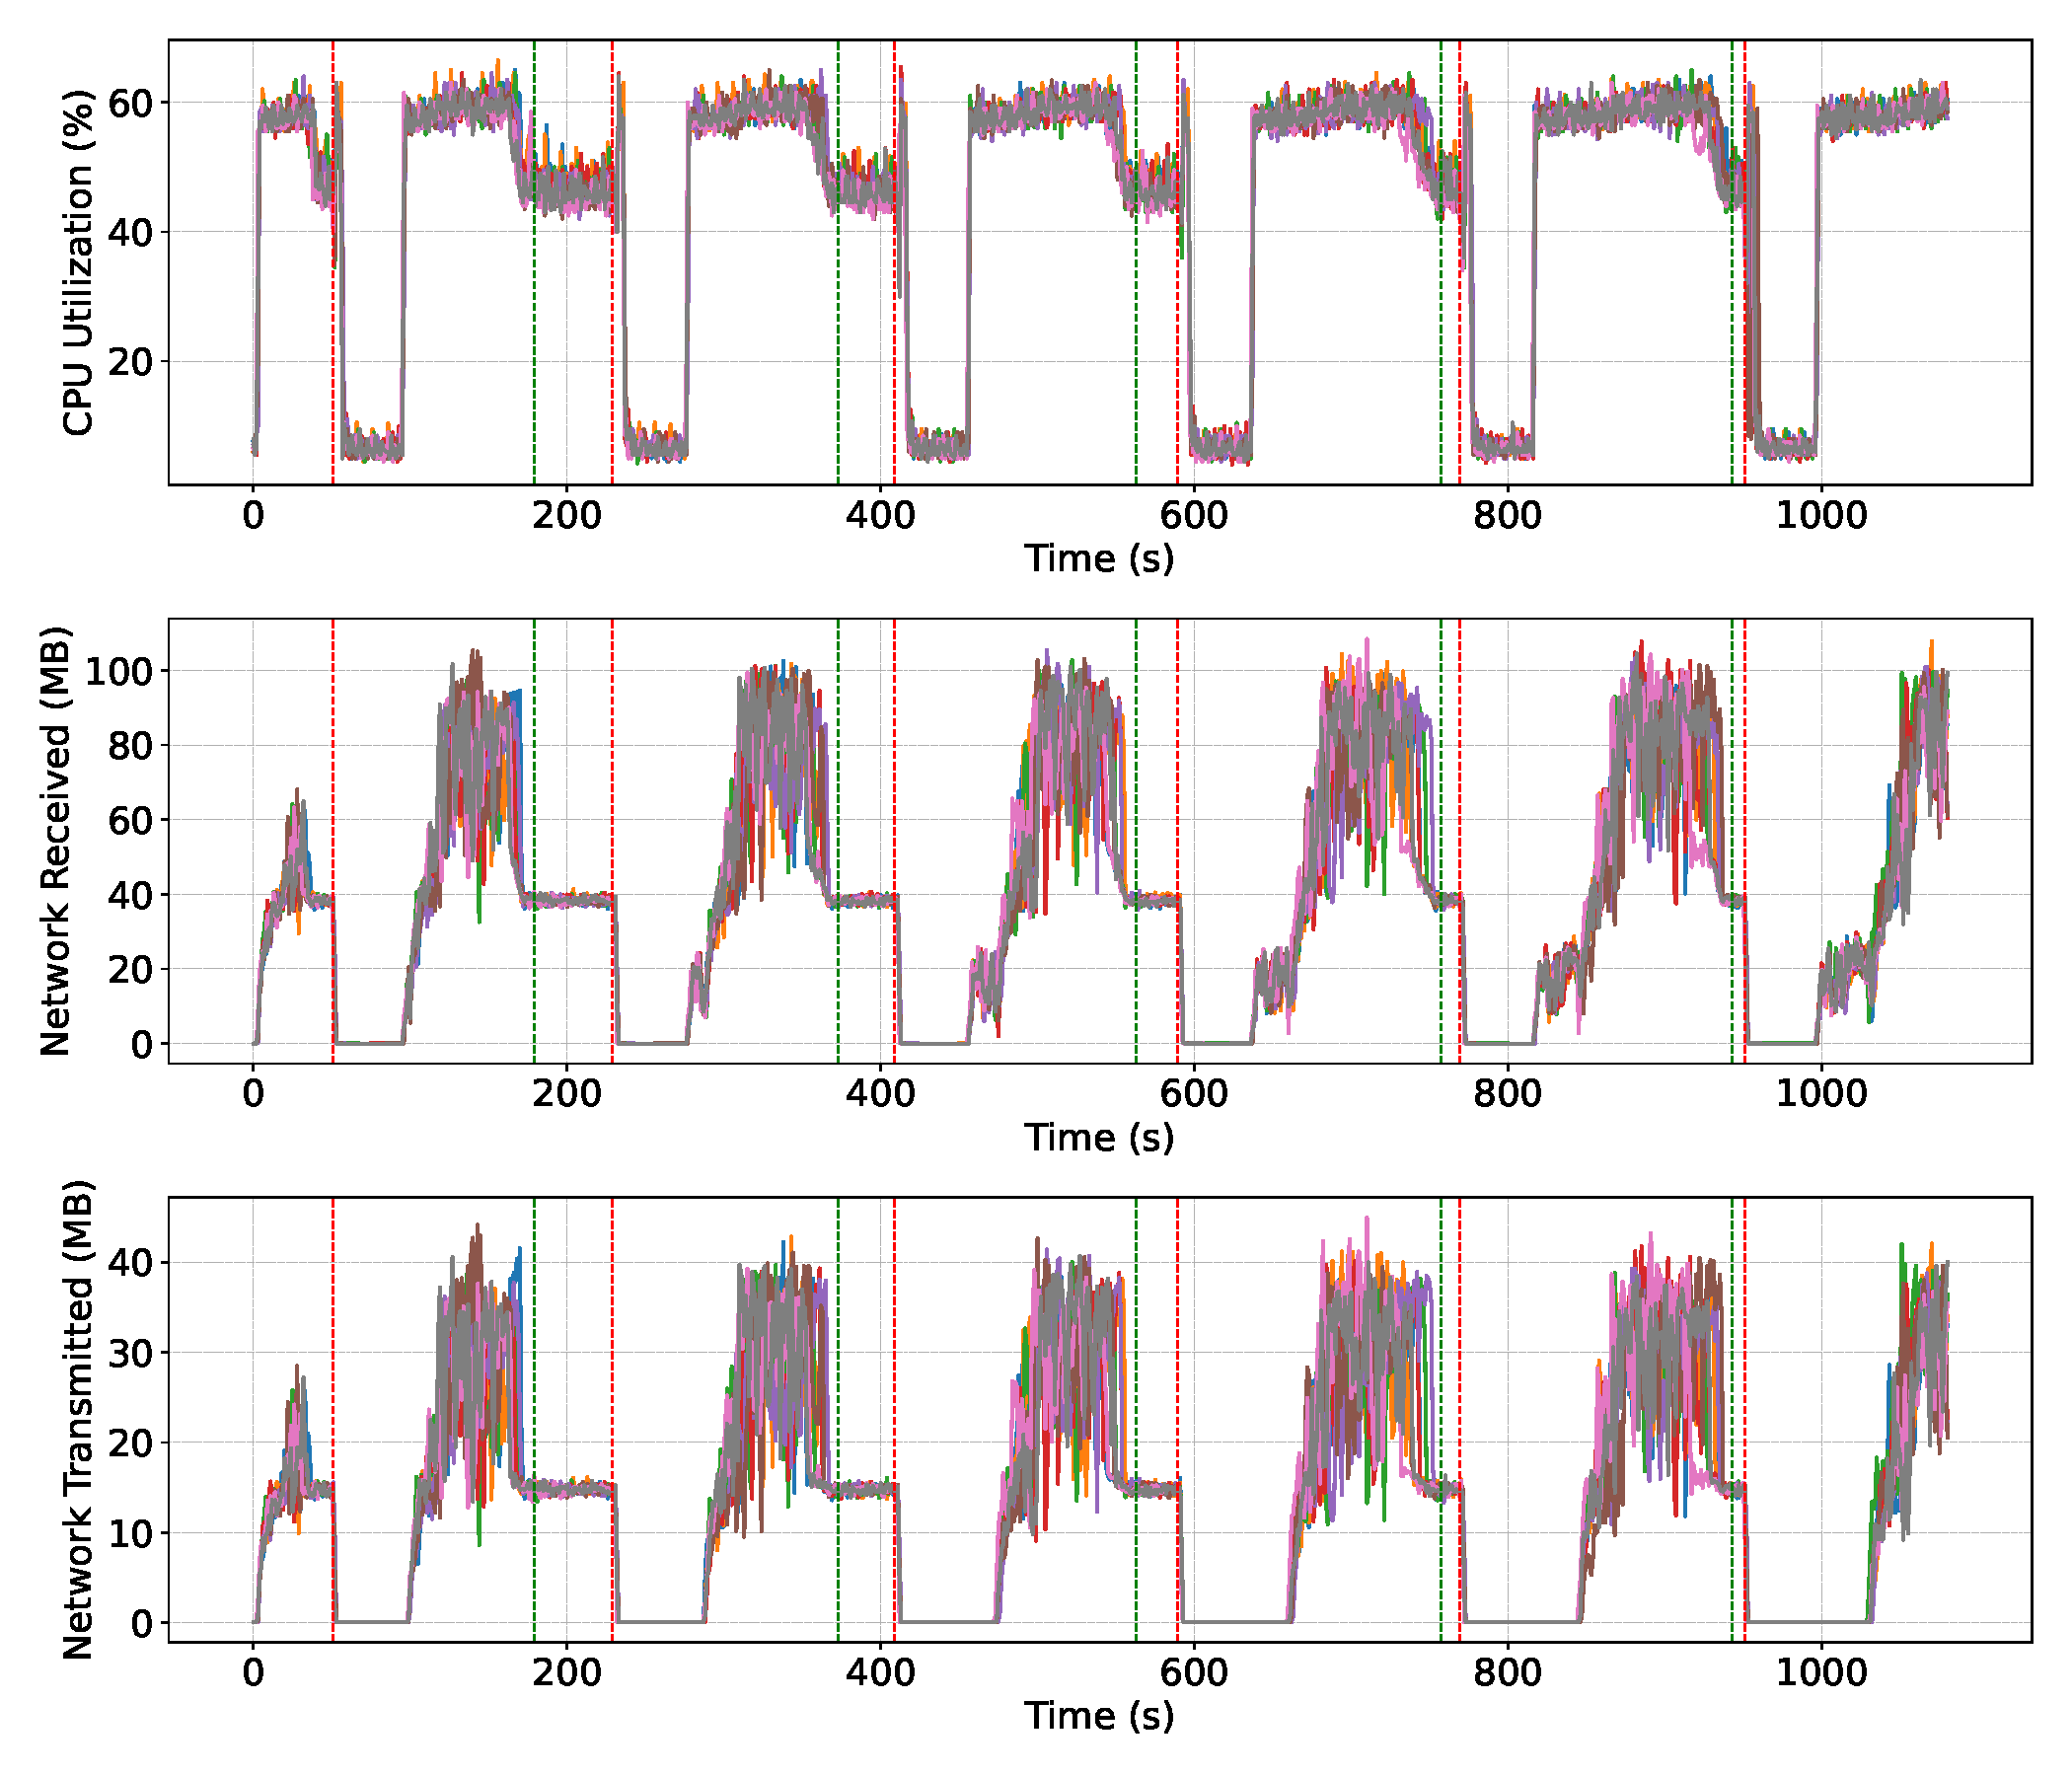
\includegraphics[width=1\textwidth]{figures/kstreams-8pods/kafka_8_pods_resources}
    \caption{\textit{Text.}}
    \label{fig:kafka-8pods-resource}
\end{figure}




\section{Benchmarking Apache Flink Fault Tolerance}\label{sec:benchmarking-apache-flink-fault-tolerance}

\subsection{Analyzing 2-Pod Failures in an 8-Pod Cluster}\label{subsec:analyzing-2-pod-failures-in-an-8-pod-cluster2}


\begin{figure}[ht]
    \centering
    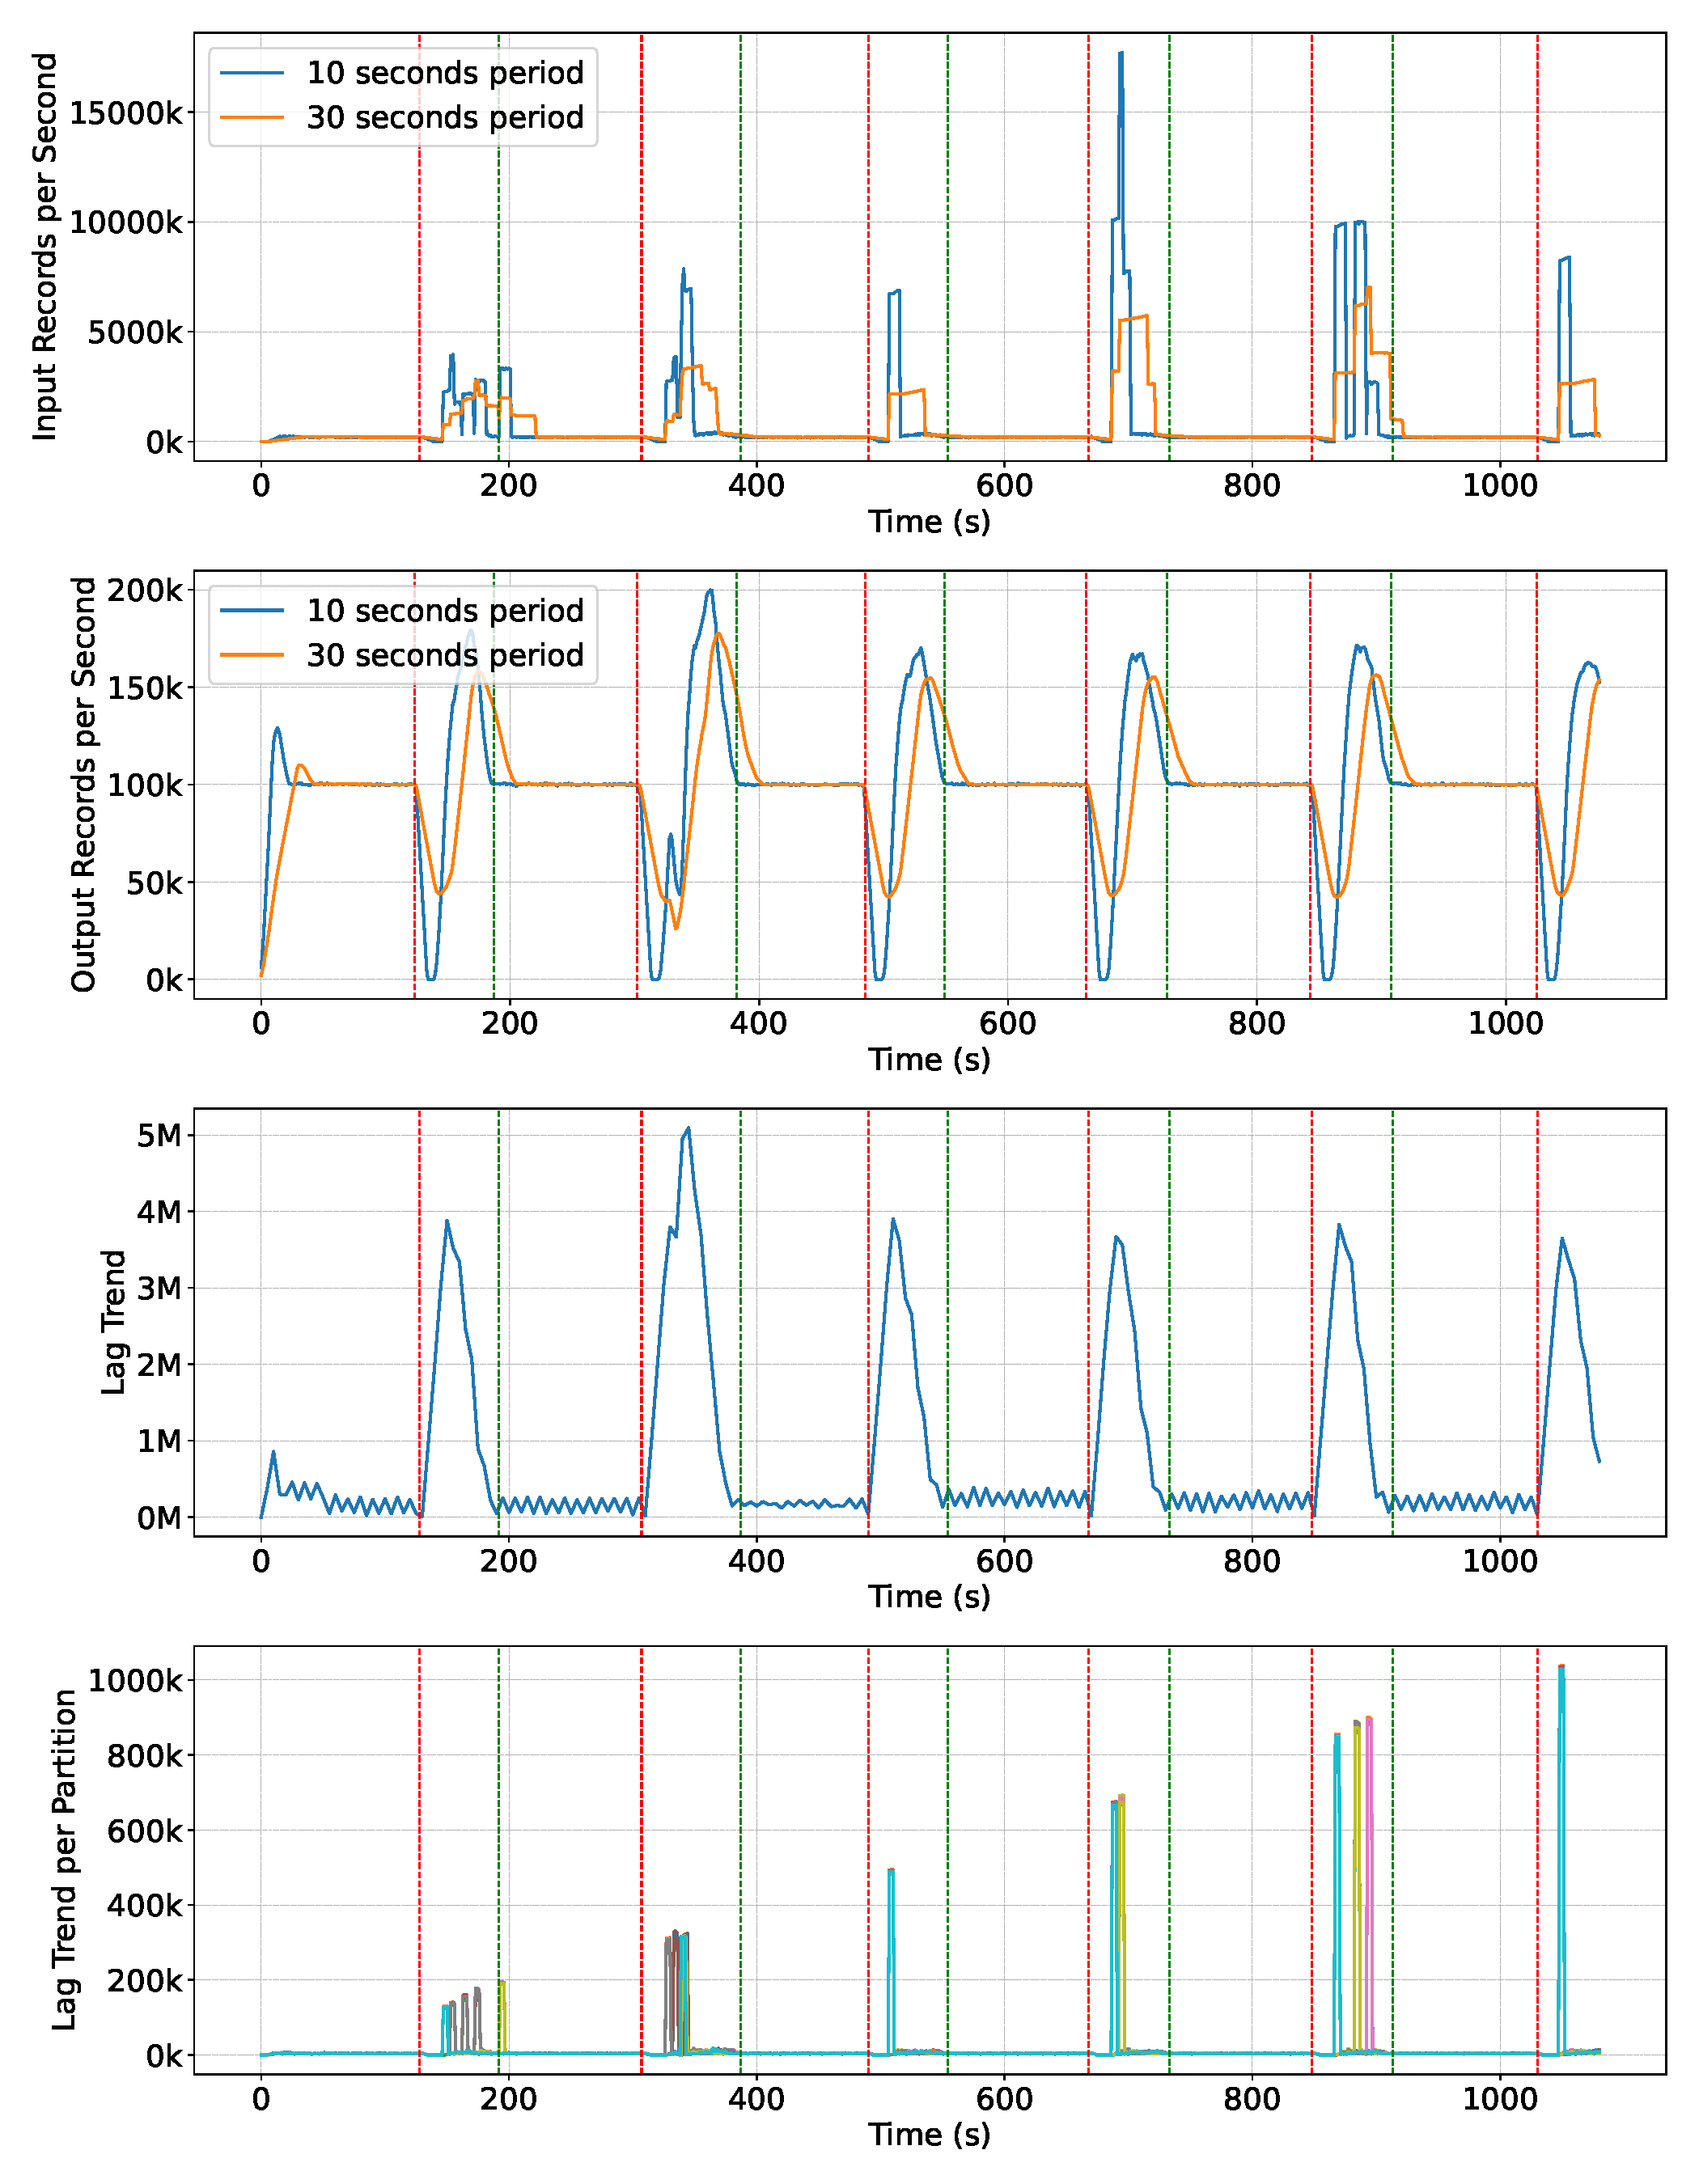
\includegraphics[width=1\textwidth]{figures/flink-2pods/flink_2_pods_plot_impact}
    \caption{\textit{Text.}}
    \label{fig:flink-2pods-impact}
\end{figure}


\begin{figure}[ht]
    \centering
    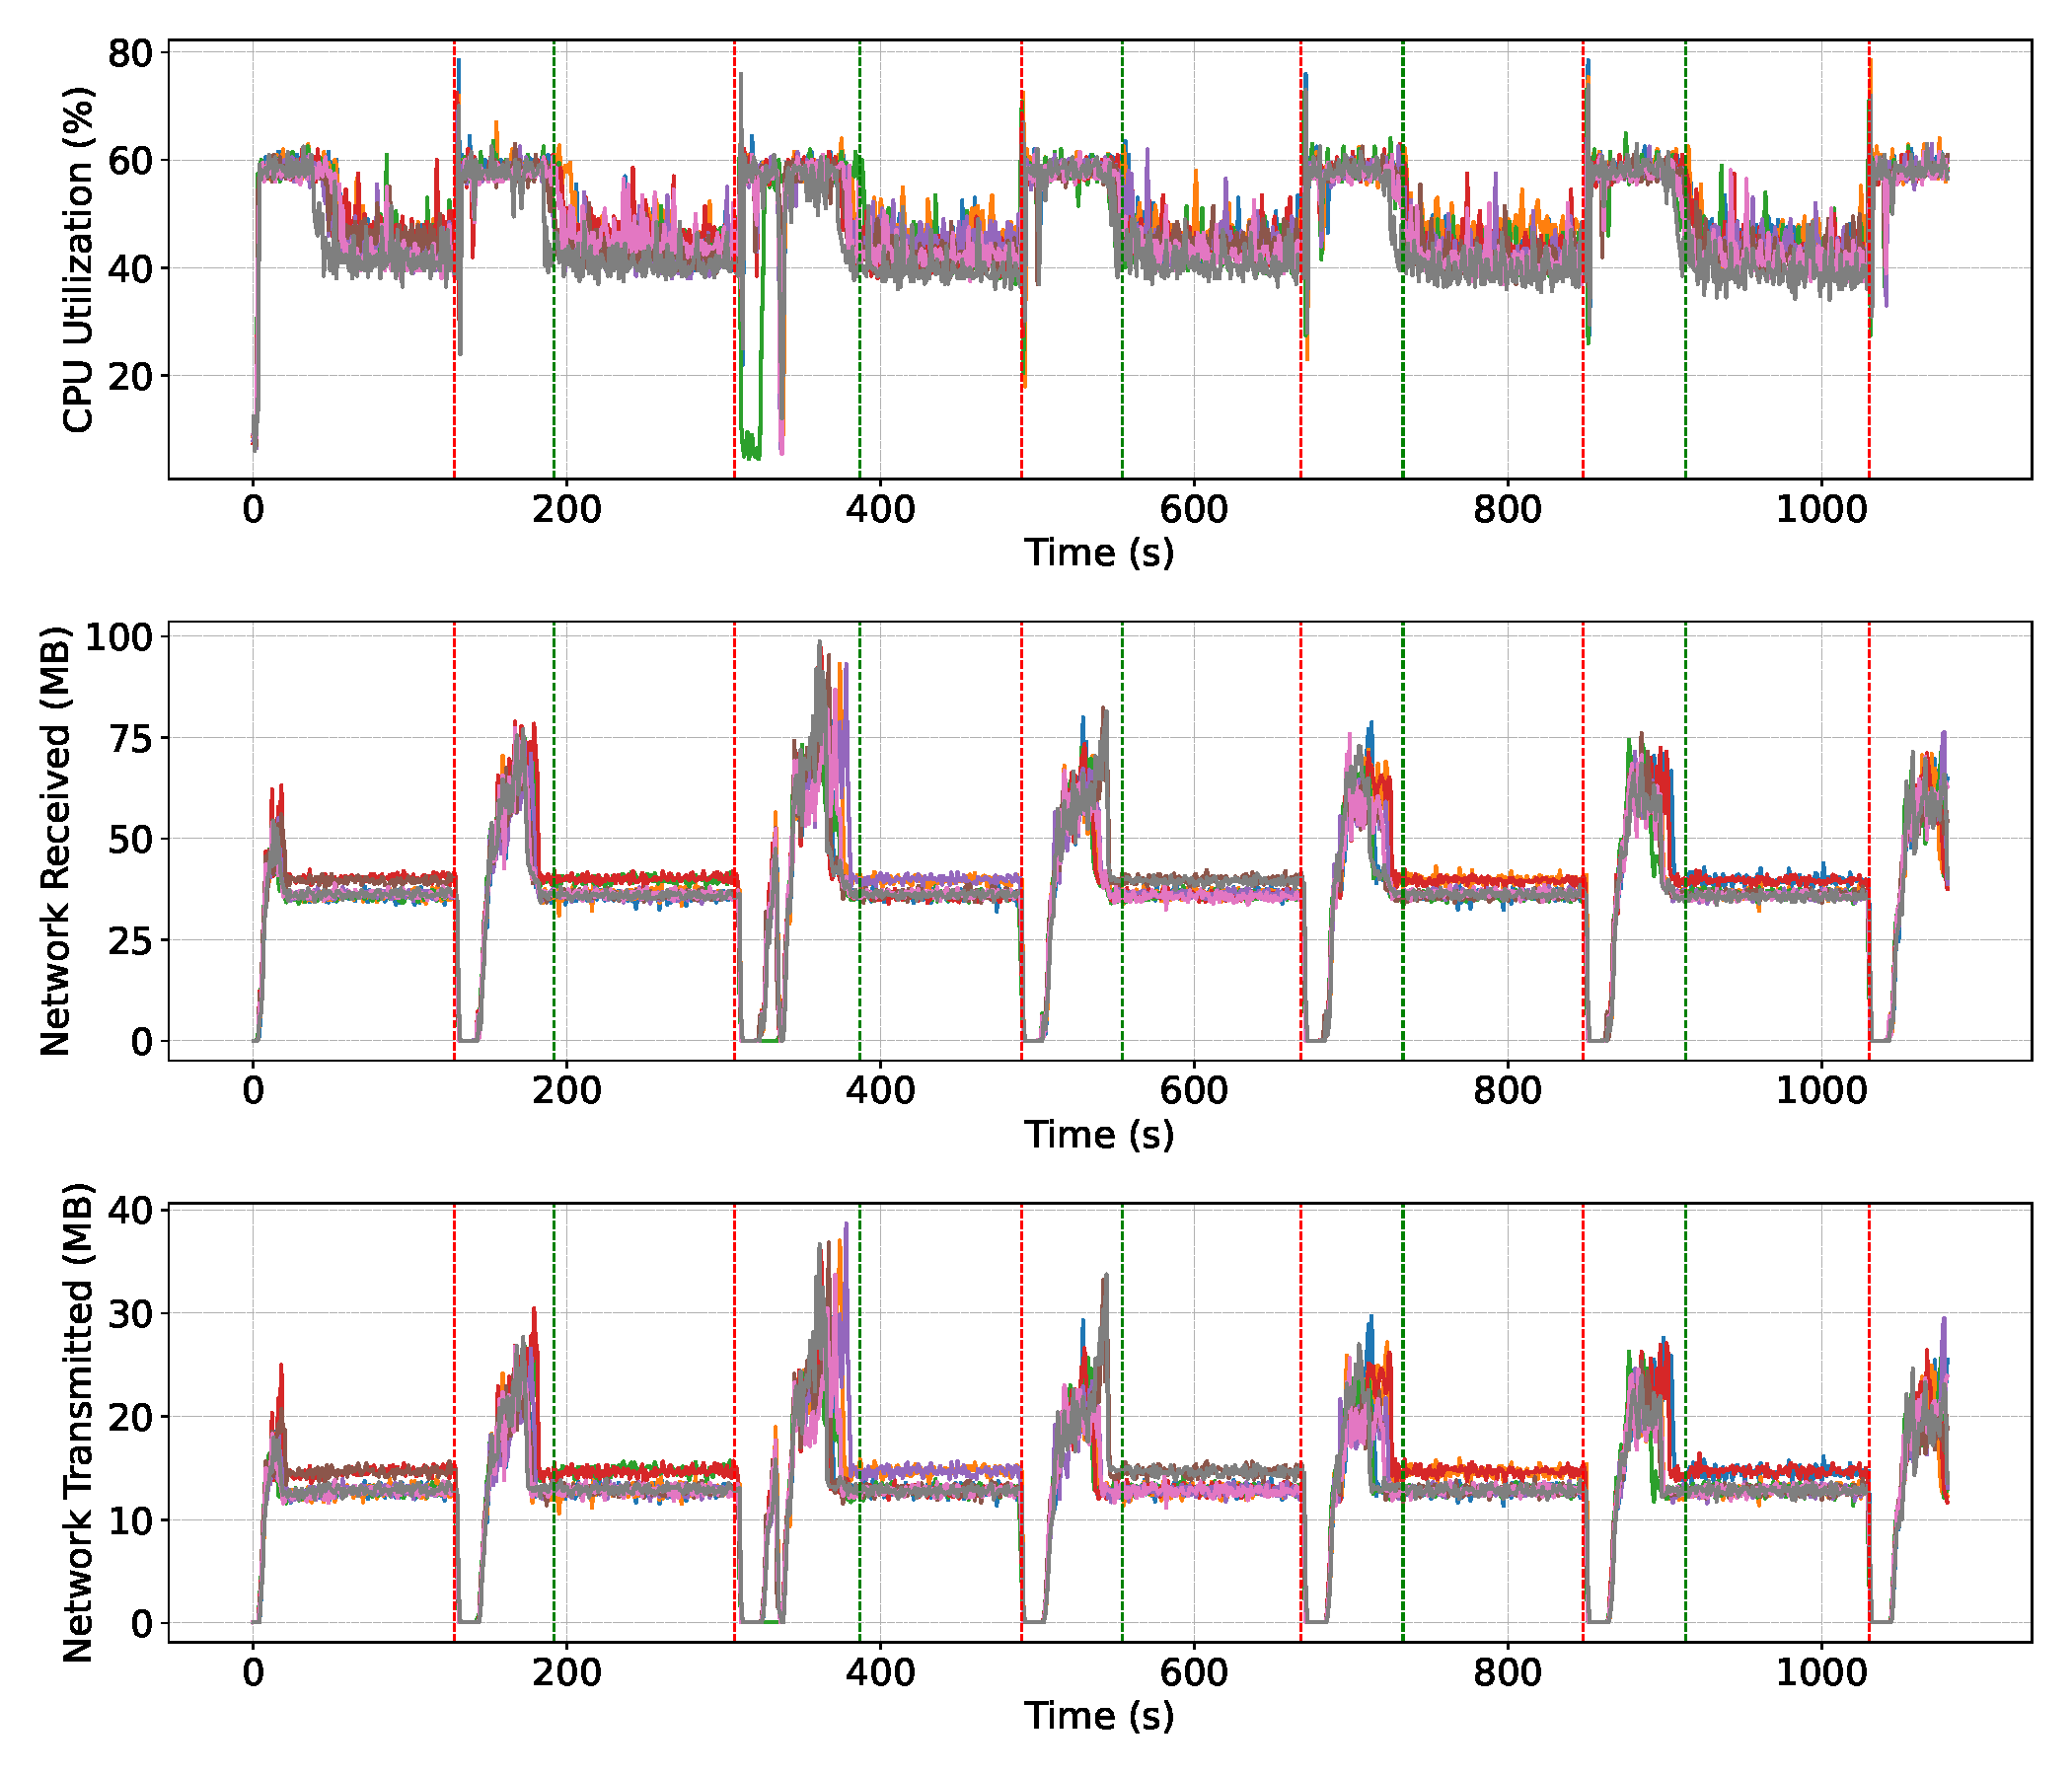
\includegraphics[width=1\textwidth]{figures/flink-2pods/flink_2_pods_resources}
    \caption{\textit{Text.}}
    \label{fig:flink-2pods-resource}
\end{figure}


\subsection{Analyzing 8-Pod Failures in an 8-Pod Cluster}\label{subsec:analyzing-8-pod-failures-in-an-8-pod-cluster2}

\begin{figure}[ht]
    \centering
    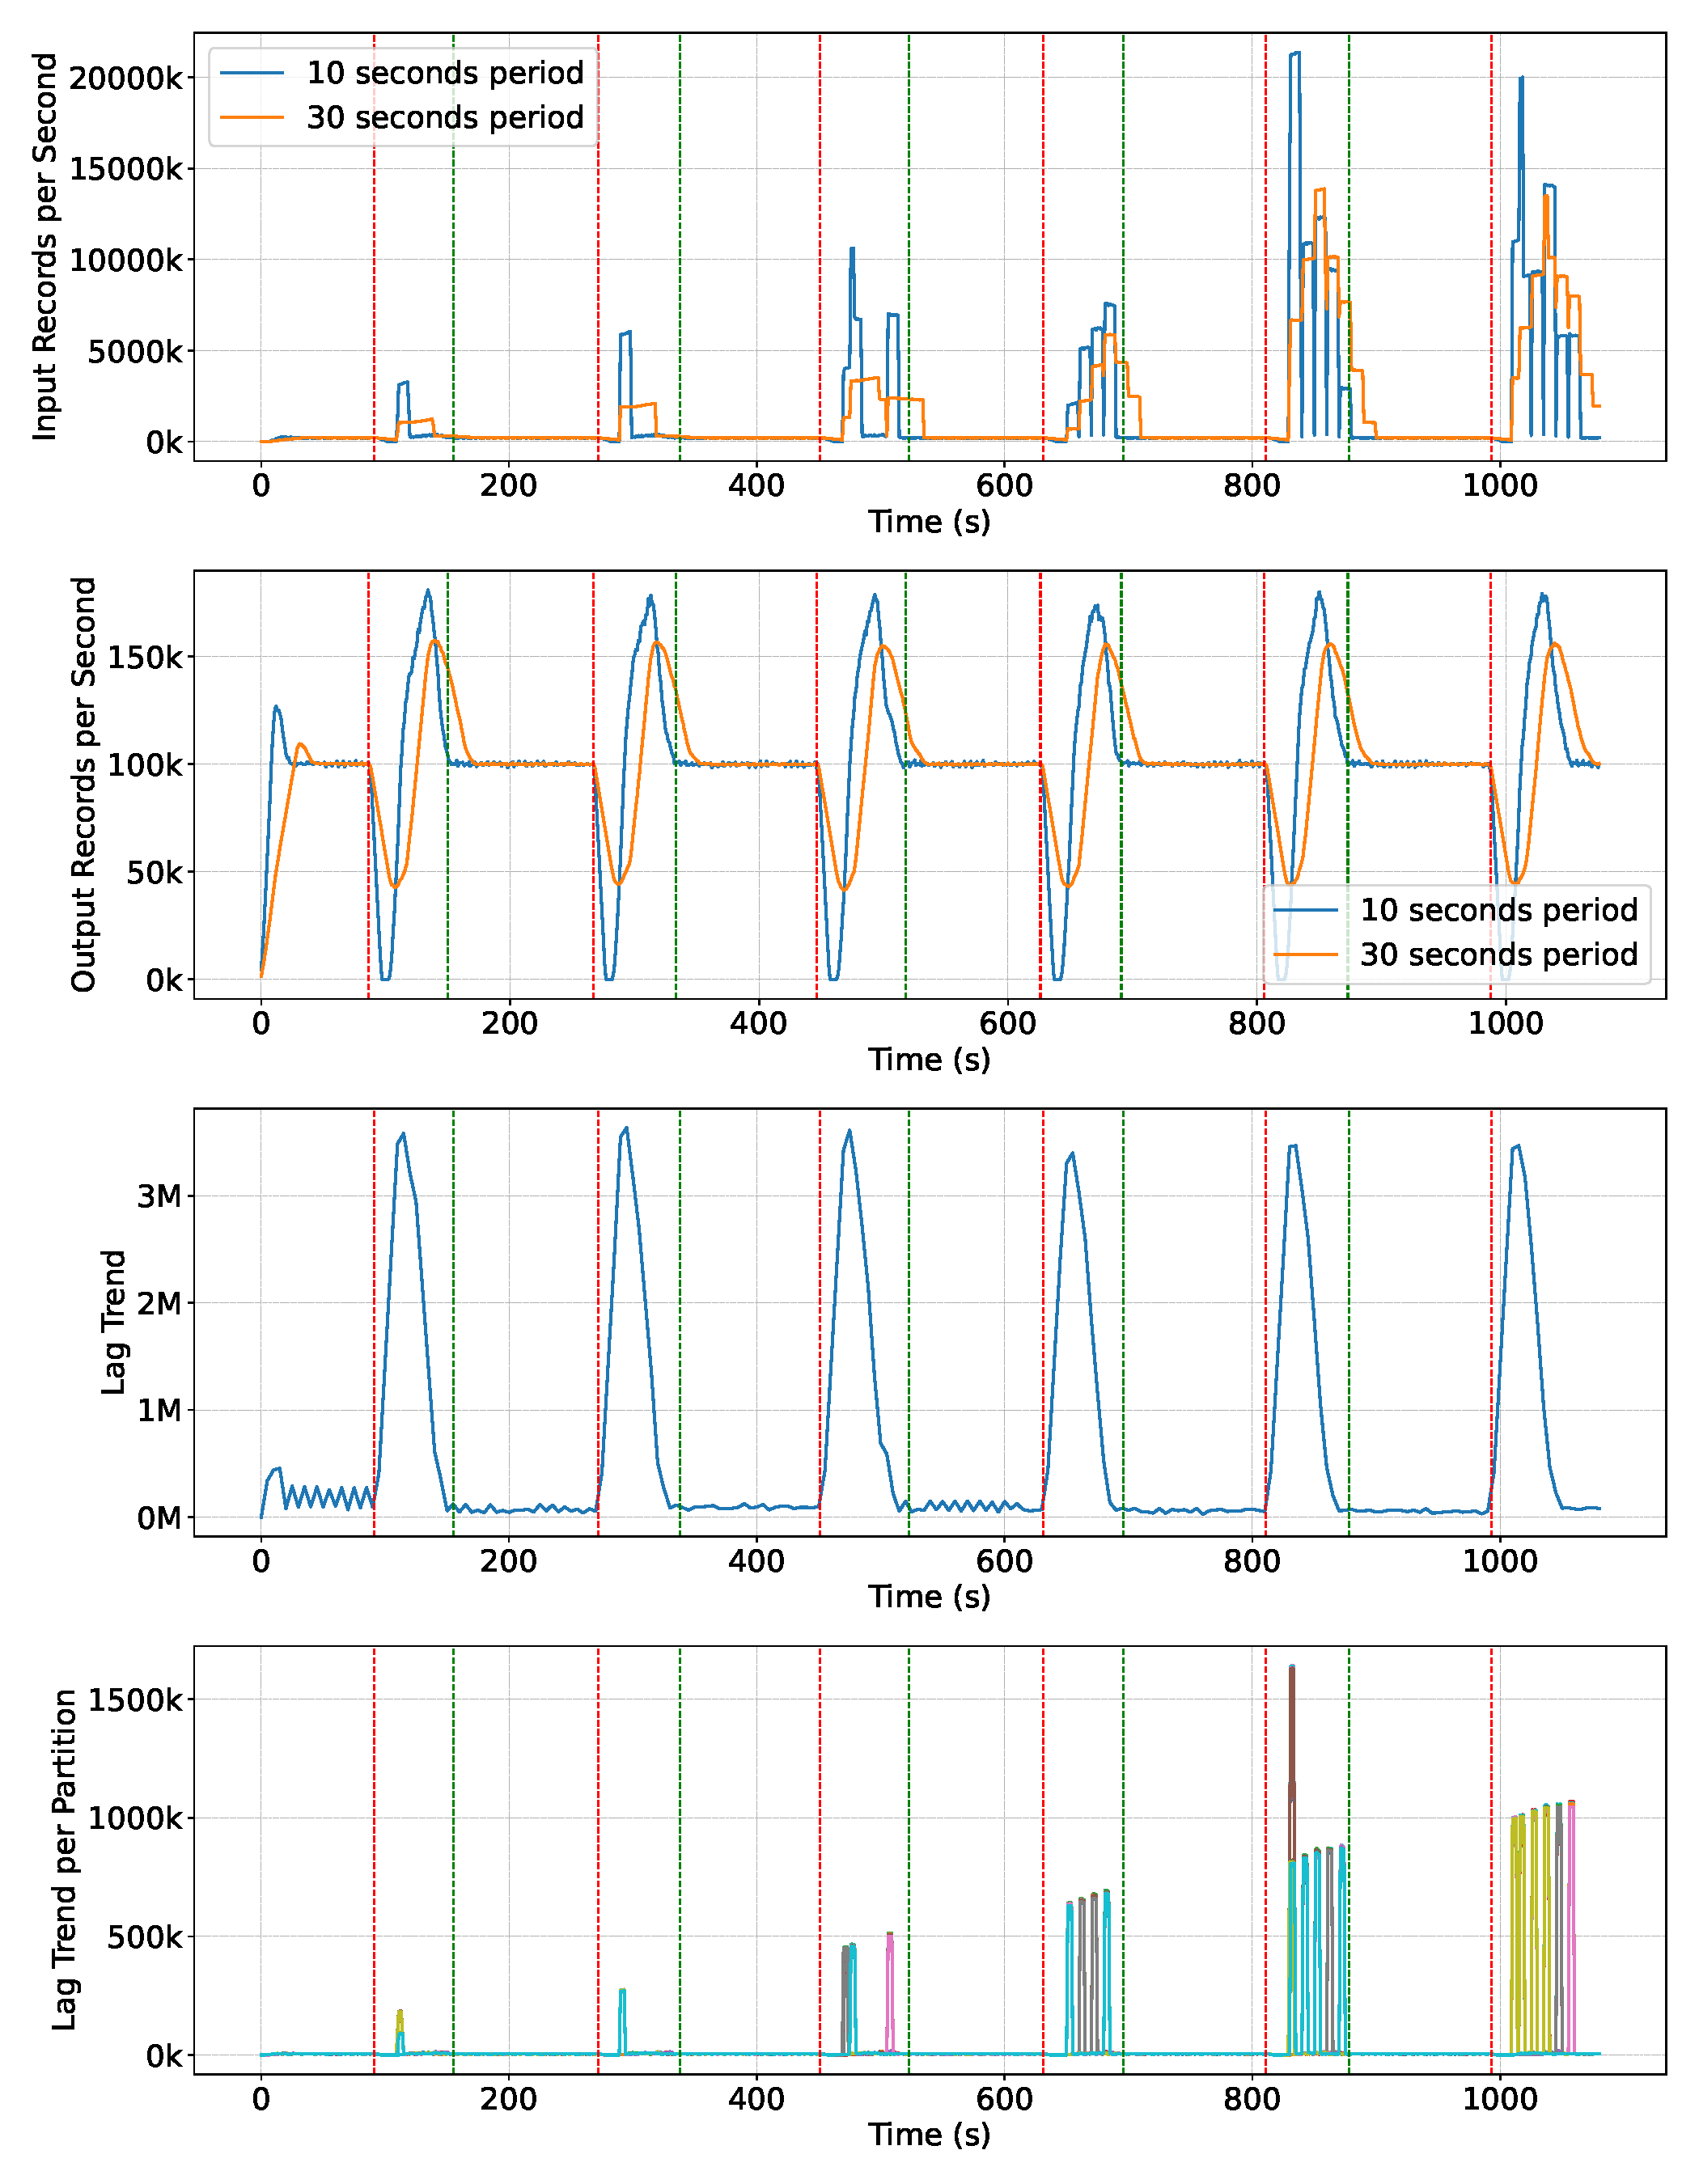
\includegraphics[width=1\textwidth]{figures/flink-8pods/flink_8_pods_plot_impact}
    \caption{\textit{Text.}}
    \label{fig:flink-8pods-impact}
\end{figure}


\begin{figure}[ht]
    \centering
    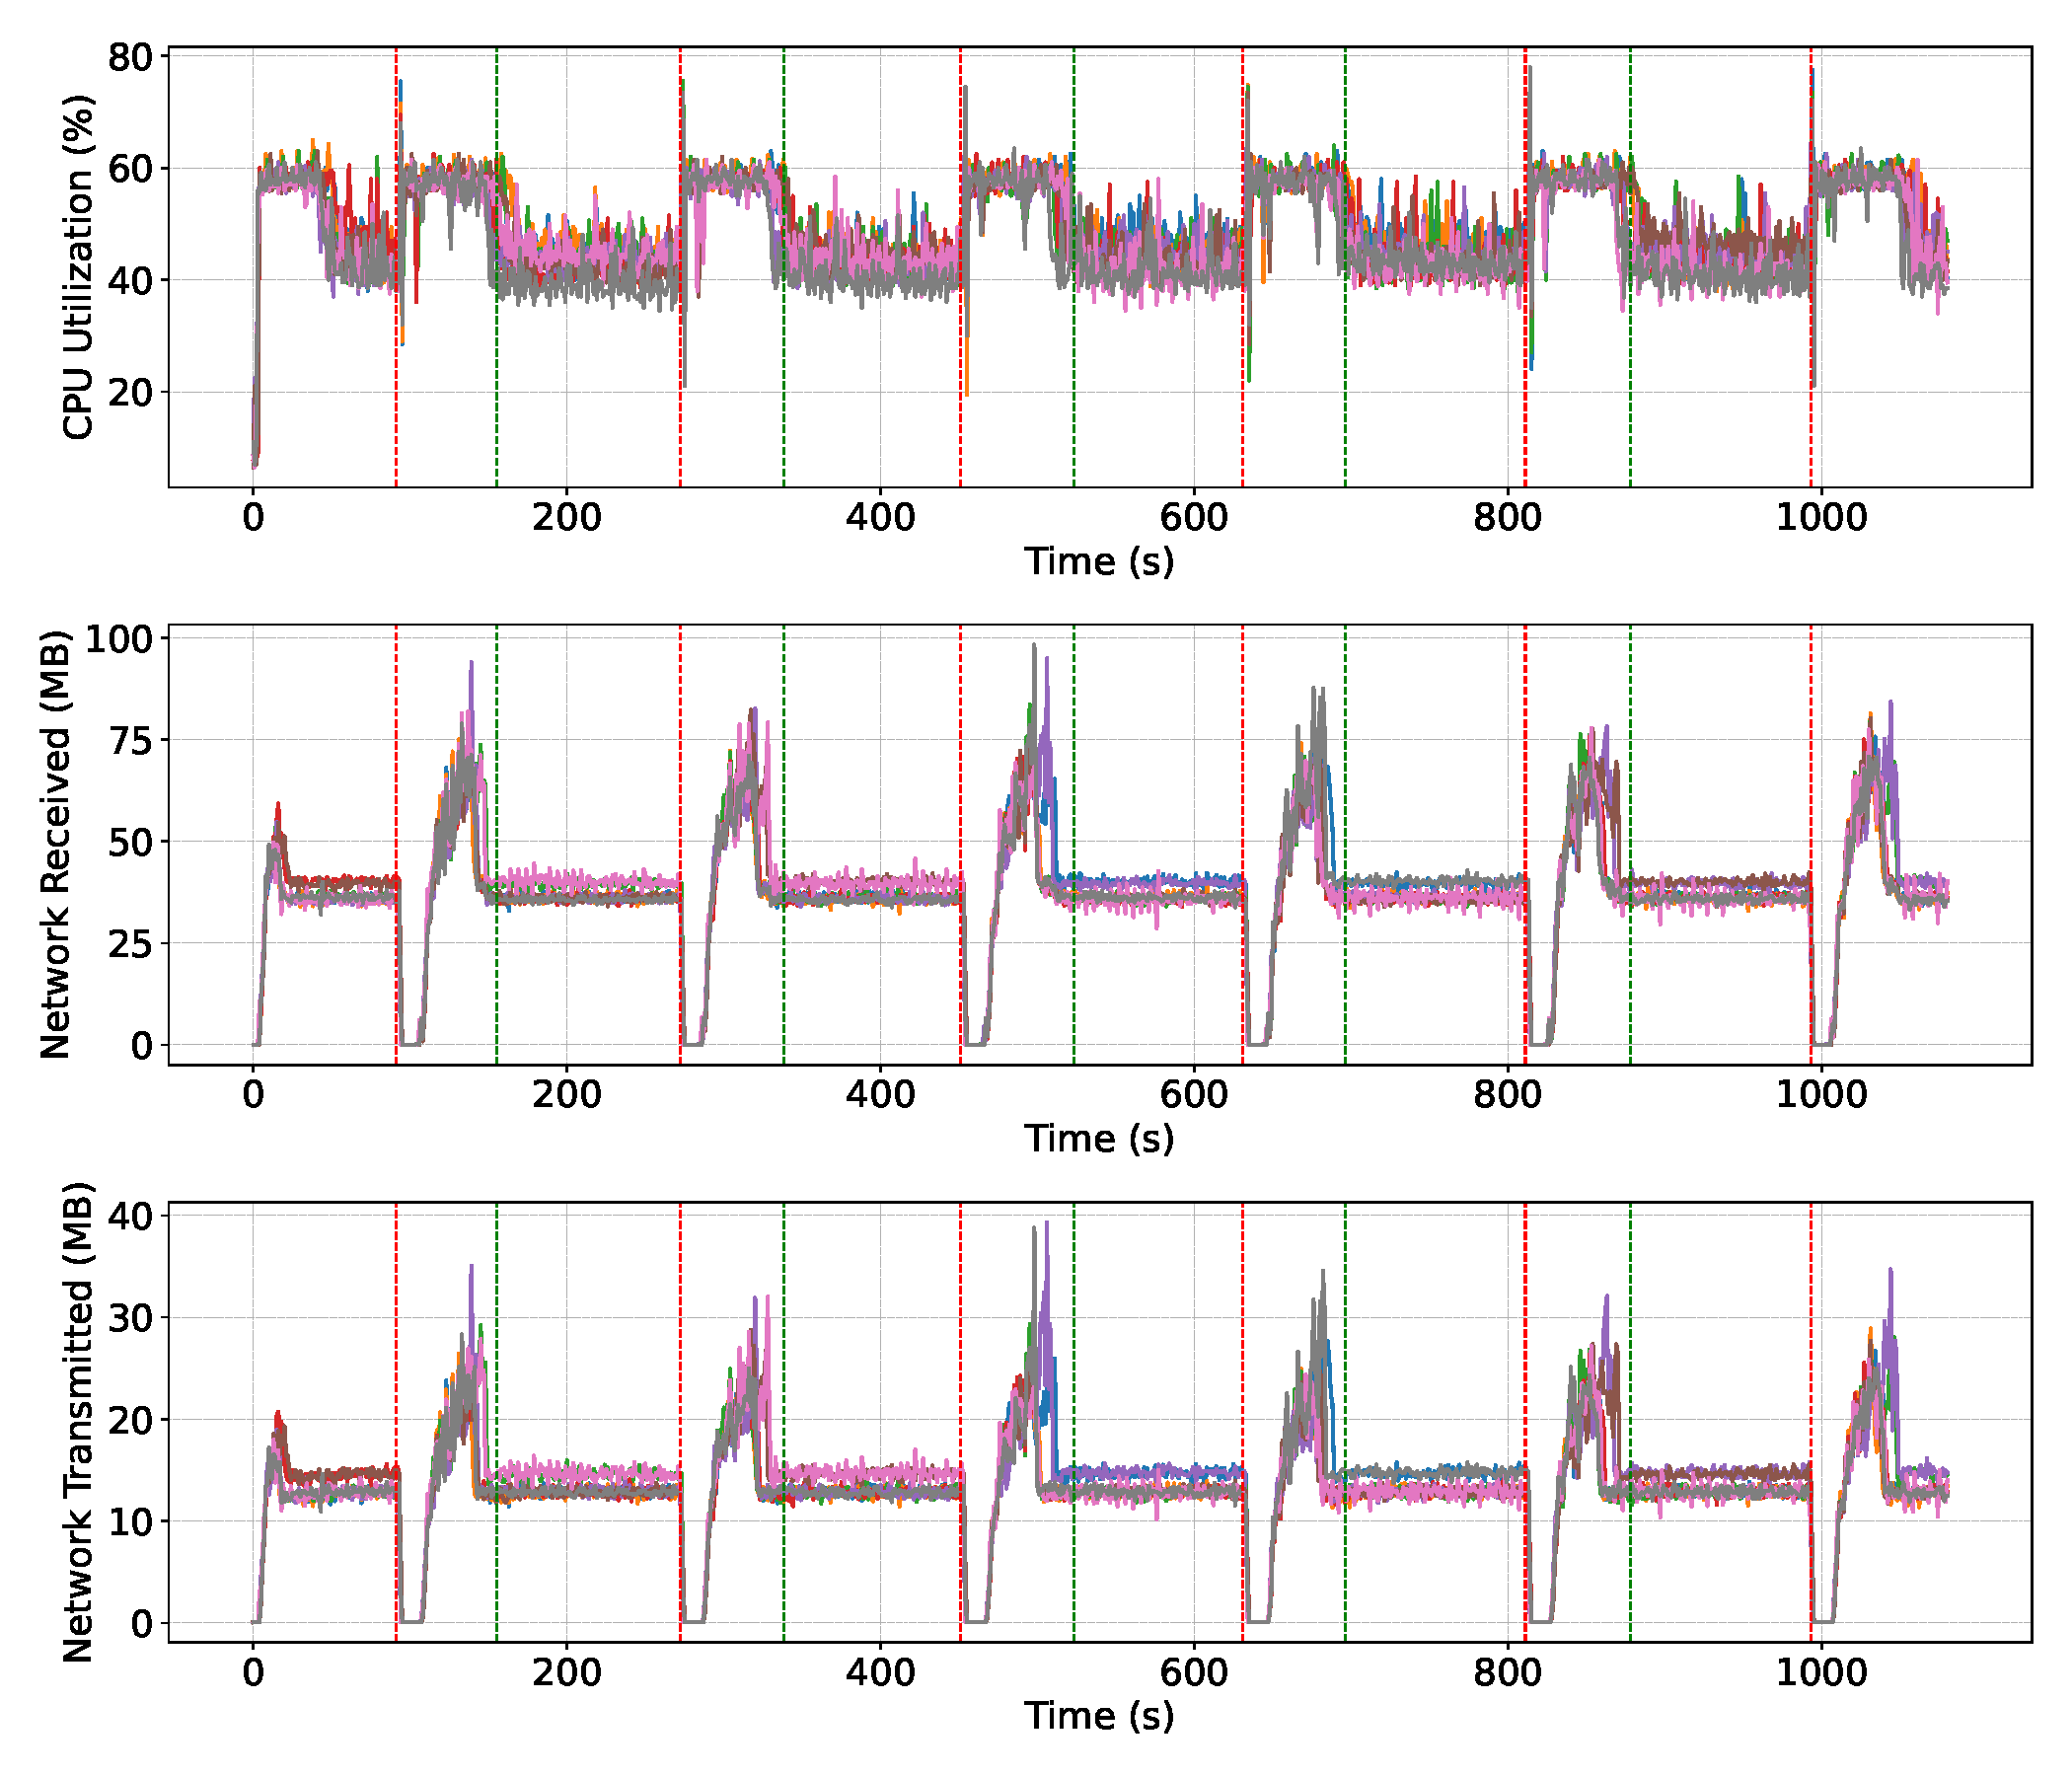
\includegraphics[width=1\textwidth]{figures/flink-8pods/flink_8_pods_resources}
    \caption{\textit{Text.}}
    \label{fig:flink-8pods-resource}
\end{figure}


\subsection{Comparative analysis}\label{subsec:comparative-analysis}

\begin{figure}[ht]
    \centering
    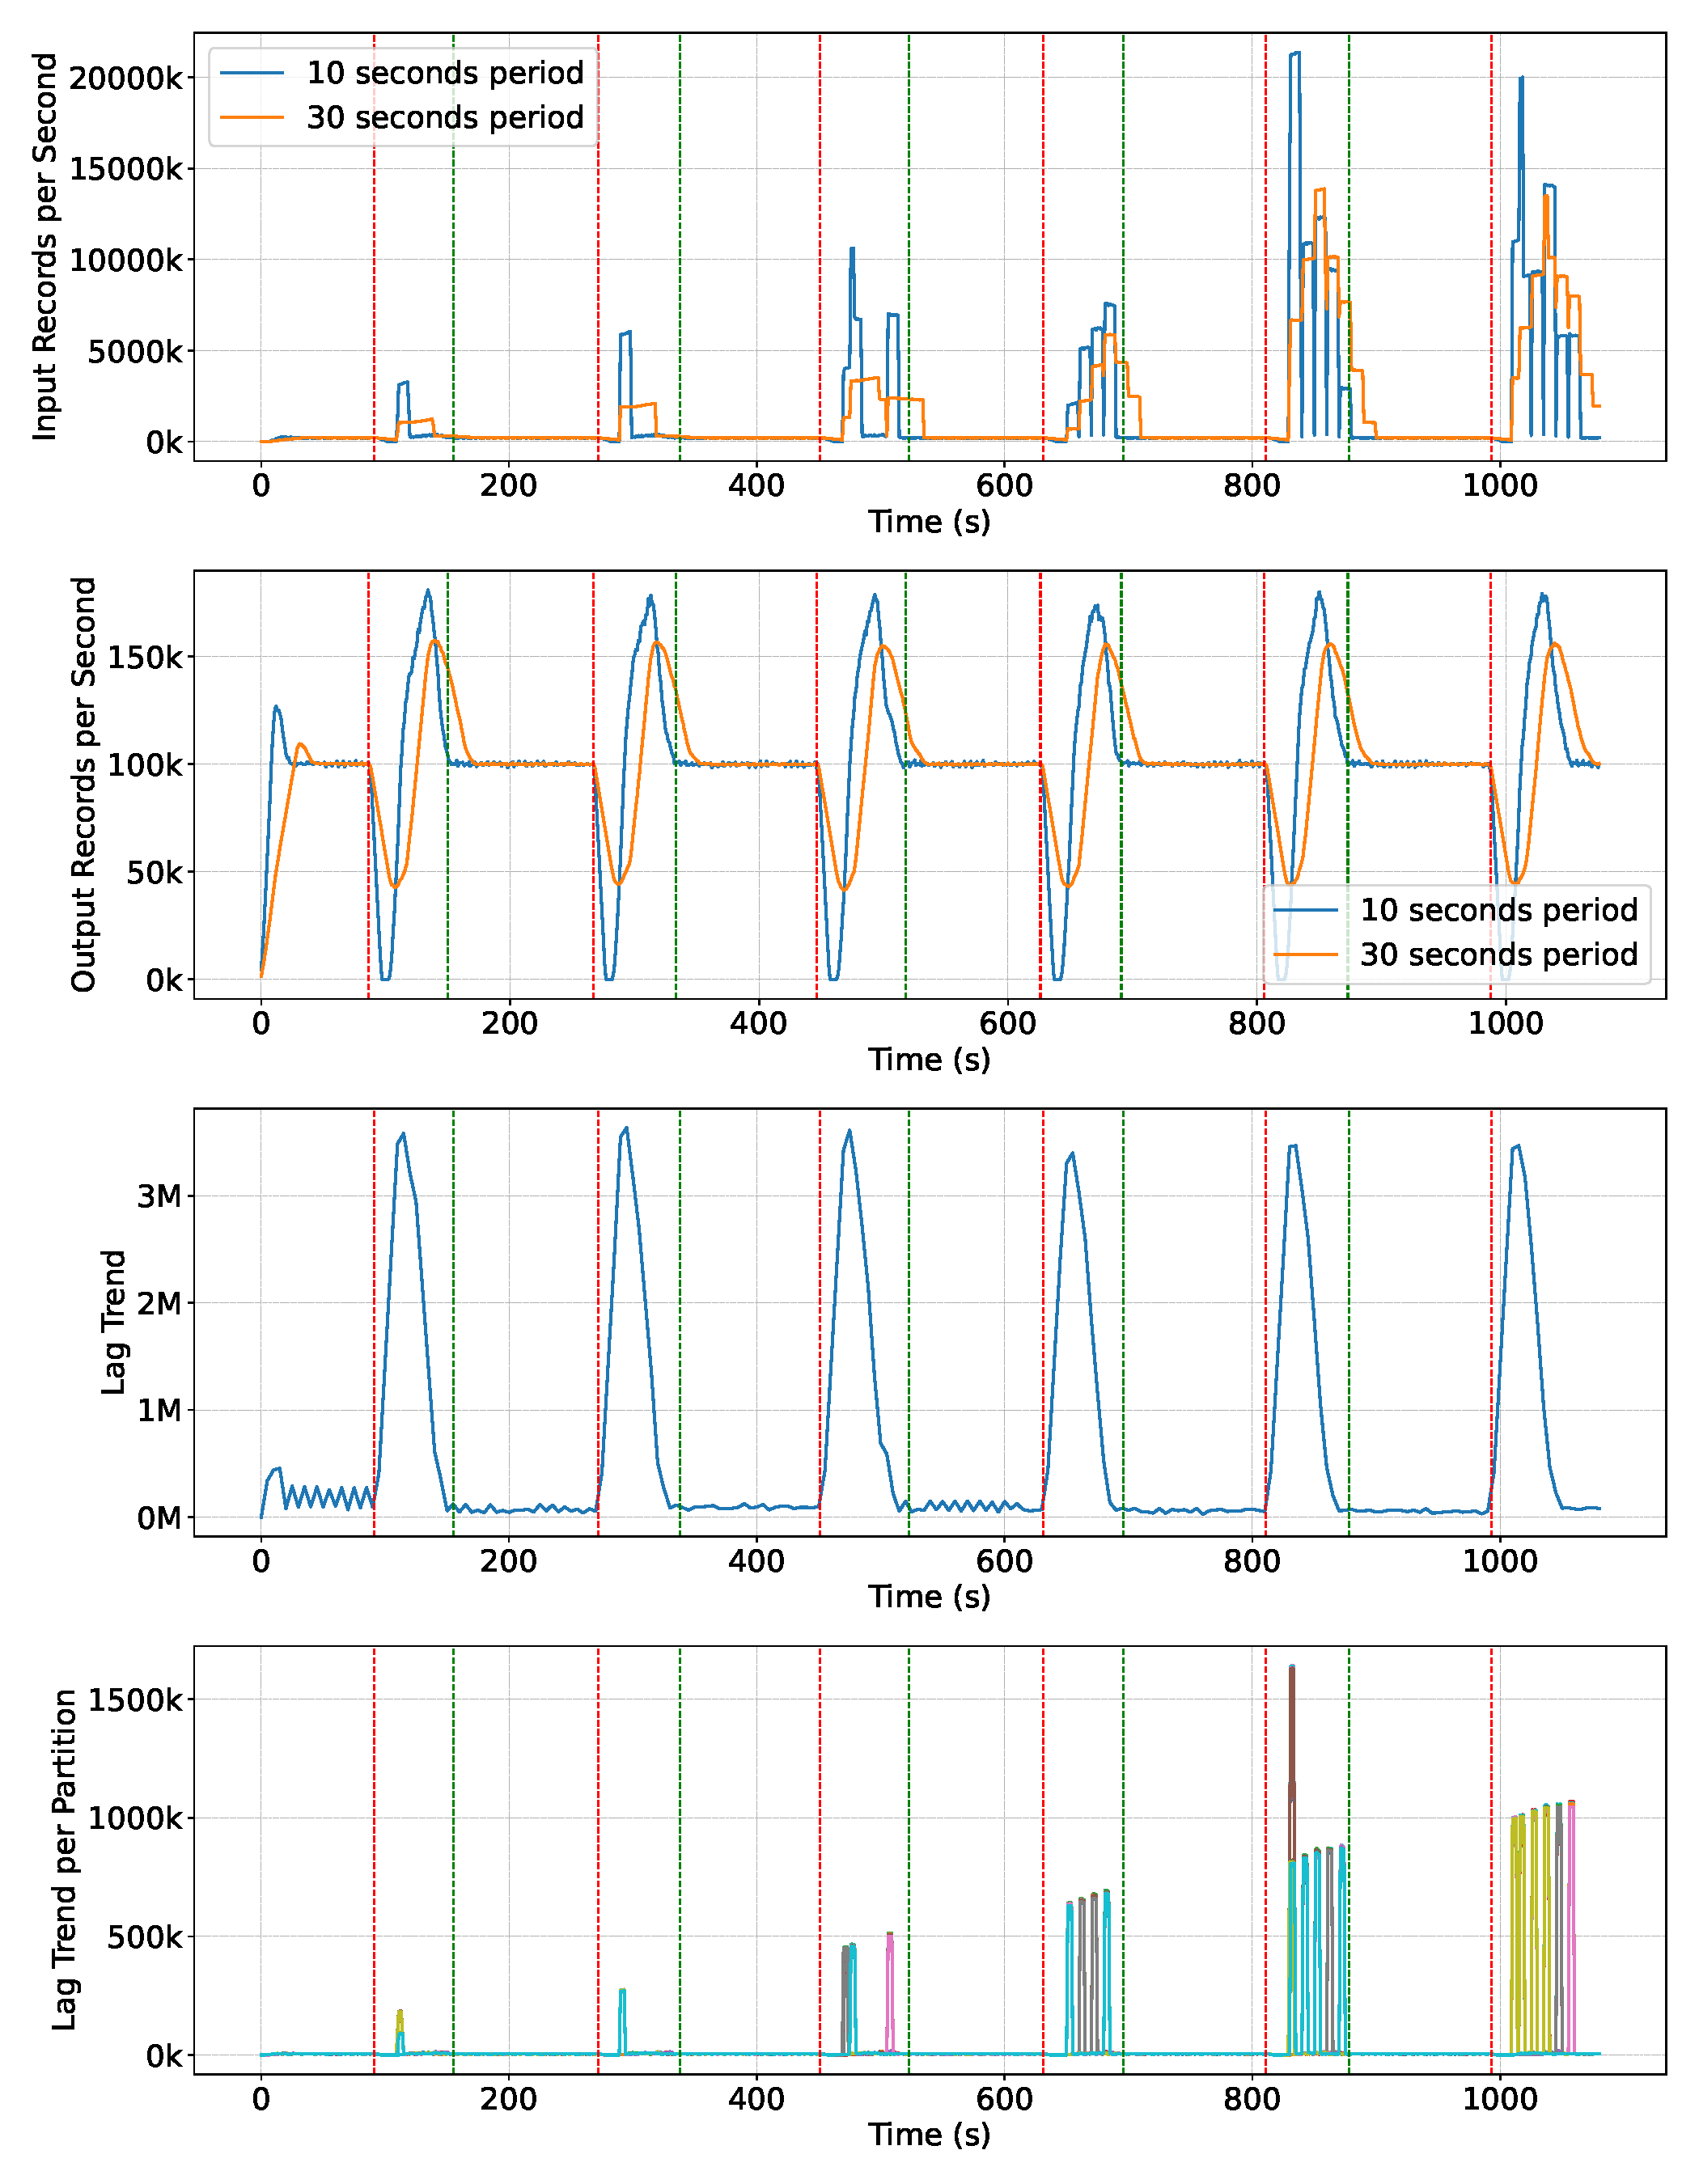
\includegraphics[width=1\textwidth]{figures/flink-8pods/flink_8_pods_plot_impact}
    \caption{\textit{Text.}}
    \label{fig:kafka-flink-input}
\end{figure}

